\section{Appendix}
\subsection{Sample Splits: Suggestion 1}
\begin{figure} [h!]
    \begin{center}
     \caption{Hypothesis 1: Intentions of the borrower countries}
    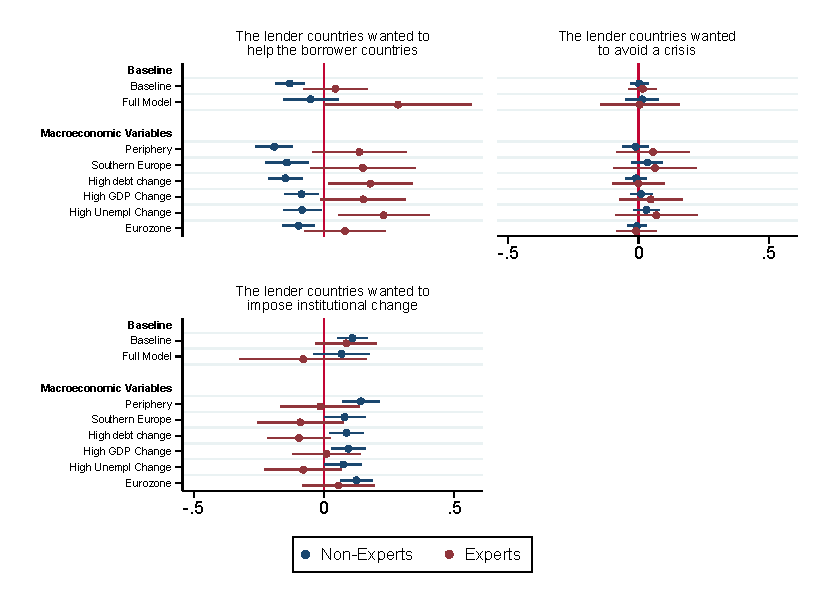
\includegraphics[scale=1.2]{Question2_samplesplits.pdf}
    \label{fig:my_label}
    \end{center}
    \tiny 
    \tablenotes{Participants were asked to assess the following statements:  Question 2.1: The lender countries wanted to help the borrowing countries Question 2.2: The lender countries wanted to help themselves avoid a crisis at home Question 2.3: The lender countries wanted to impose institutional change upon the borrower countries }
\end{figure}
\begin{figure}[h!]
    \begin{center}
     \caption{Hypothesis 4: Emotions of program countries}
    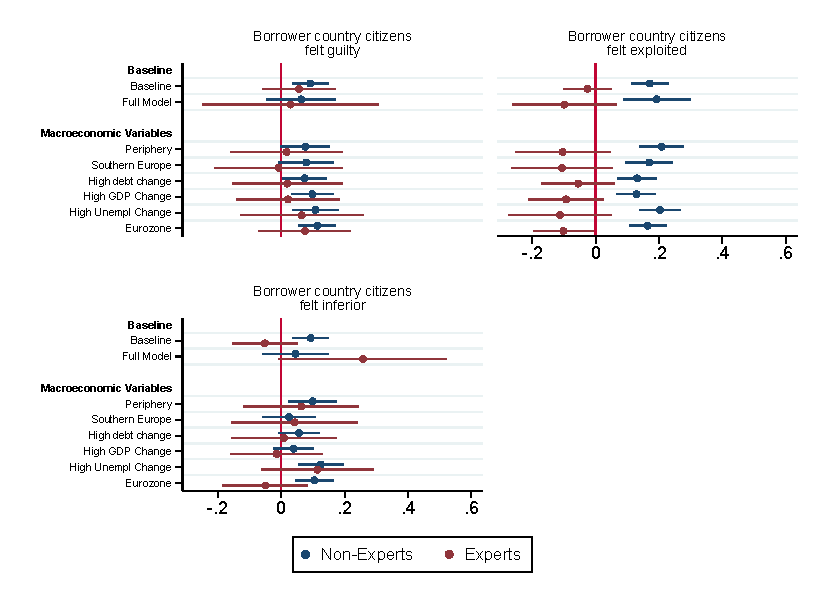
\includegraphics[scale=1.2]{Question51_samplesplits.pdf}
    \label{fig:my_label}
    \end{center}
    \tiny 
     \tablenotes{Question 5.1: The rescue experience made many citizens in the borrower countries feel guilty; Question 5.2: The rescue experience made many citizens in the borrower countries feel exploited; Question 5.3: The rescue experience made many citizens in the borrower countries feel inferior} 
\end{figure}
\begin{figure}[h!]
    \begin{center}
     \caption{Hypothesis 4: Emotions of non-program countries and repayment of outstanding debt}
    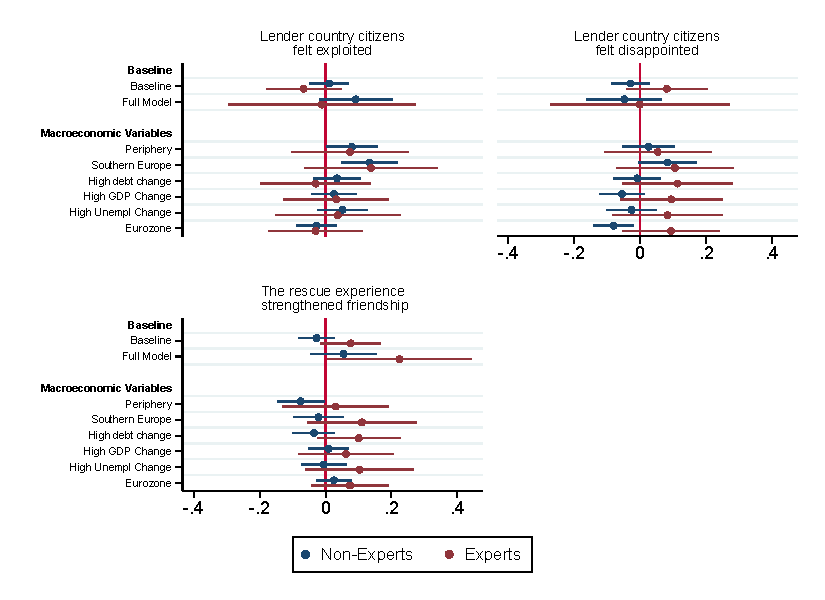
\includegraphics[scale=1.2]{Question52_samplesplits.pdf}
    \end{center}
    \tiny
     \tablenotes{Question 5.4: The rescue experience made many citizens in the lender countries feel exploited; Question 5.5 The rescue experience made many citizens in the lender countries feel disappointed Question 5.6: The rescue experience strengthened friendships between citizens Question 7: Greece will fully pay back it's debt}
\end{figure}
\begin{figure}[h!]
    \begin{center}
     \caption{Hypothesis 2 and 3: Who initiated and benefited from the rescue program}
    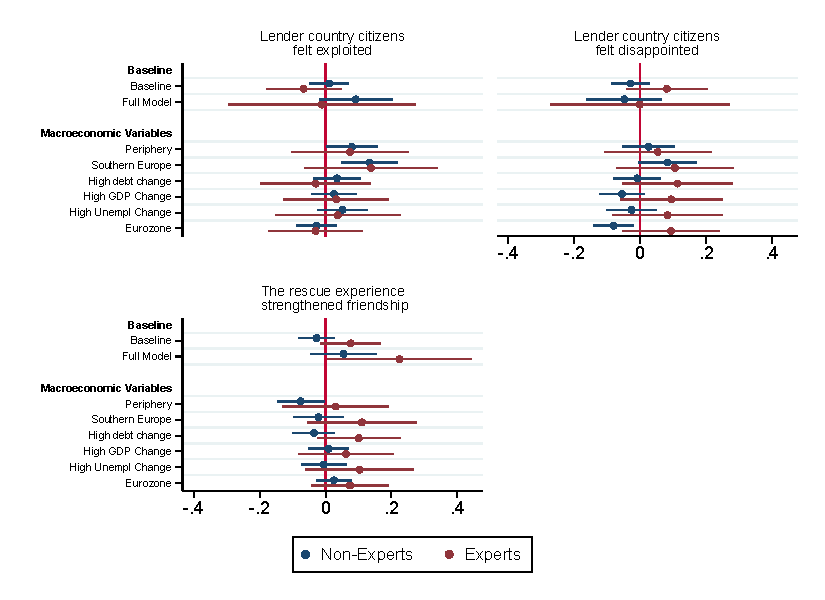
\includegraphics[scale=1.2]{Question52_samplesplits.pdf}
    \end{center}
    \tiny
    \tablenotes{Question 3: Who was the driving force behind signing the memorandum; Question 4: Who was the main beneficiary of the program; Question 7: Who primarily benefited from the loans to Greece}
\end{figure}


\begin{figure}[h!]
\caption{Hypothesis 1: Intentions of the lender countries}
    \begin{minipage}{0.5\textwidth}

    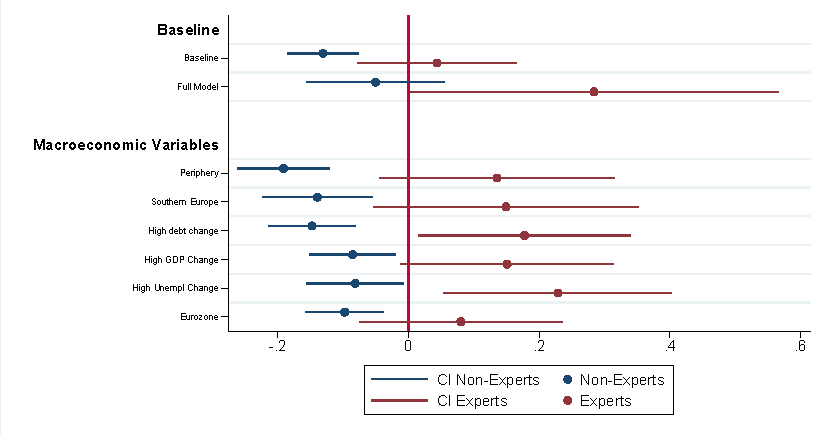
\includegraphics[scale=0.65]{QuestionS_1201.pdf}
    \footnotesize{
     \subcaption{Question 2.1}}
\end{minipage}
\begin{minipage}{0.5\textwidth}
    
    
    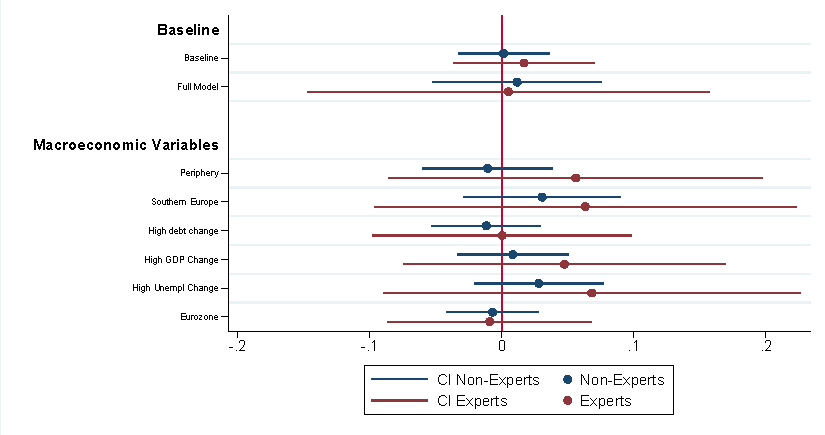
\includegraphics[scale=0.65]{QuestionS_1202.pdf}
        \footnotesize{
        \subcaption{Question 2.2} }
\end{minipage} 
 \begin{minipage}{0.5\textwidth}
  
    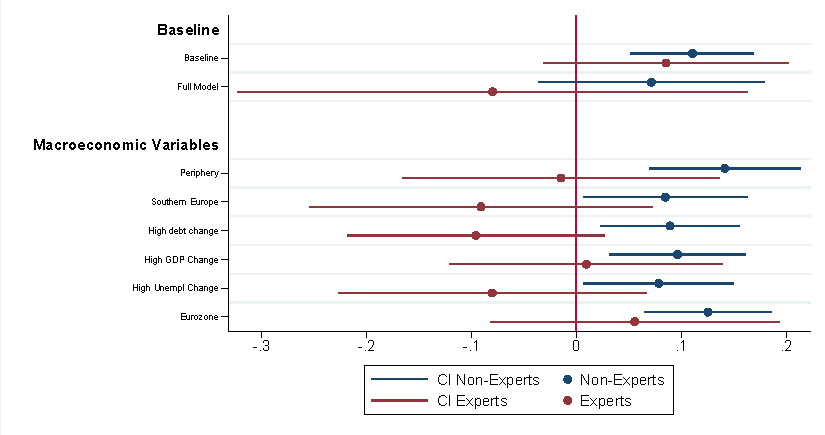
\includegraphics[scale=0.65]{QuestionS_1203.pdf}
    \footnotesize{
     \subcaption{Question 2.3}}
    \label{fig:my_label}
    \end{minipage}
     \begin{minipage}{0.5\textwidth}
         \end{minipage}
         \vskip 0.3cm
             \tiny 
    \tablenotes{Participants were asked to assess the following statements:  Question 2.1: The lender countries wanted to help the borrowing countries;  Question 2.2: The lender countries wanted to help themselves avoid a crisis at home; Question 2.3: The lender countries wanted to impose institutional change upon the borrower countries }

\end{figure} 



\begin{figure}[h!]
\caption{Hypothesis 4: Emotions evoked among citizens }
    \begin{minipage}{0.5\textwidth}
    
    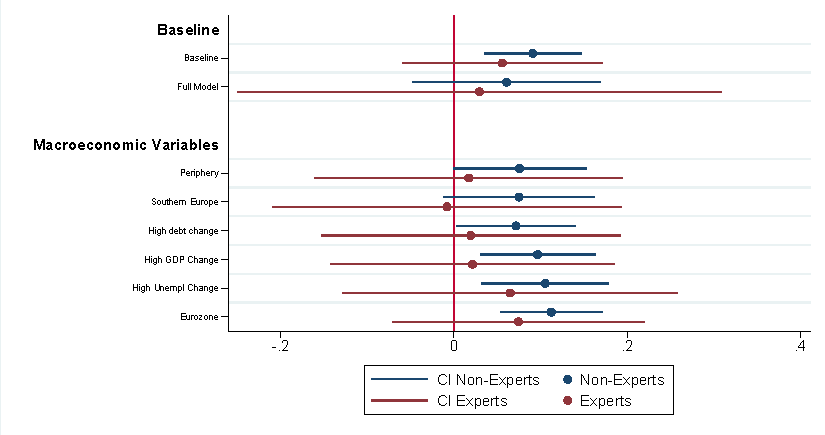
\includegraphics[scale=0.65]{QuestionS_1501.pdf}
    \footnotesize{
     \subcaption{Question 5.1} }
\end{minipage}
\begin{minipage}{0.5\textwidth}
    \centering
    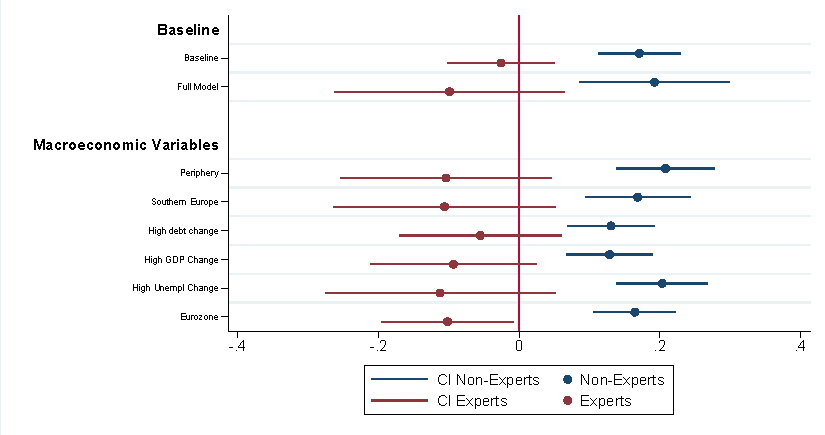
\includegraphics[scale=0.65]{QuestionS_1502.pdf}
    \footnotesize{
      \subcaption{Question 5.2}}
\end{minipage} 
 \begin{minipage}{0.5\textwidth}
    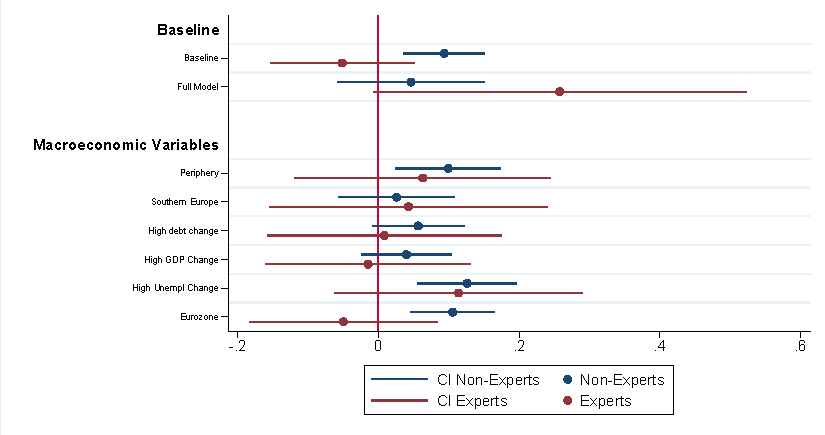
\includegraphics[scale=0.65]{QuestionS_1503.pdf}
    \footnotesize{
     \subcaption{Question 5.3}}
    \label{fig:my_label}
    \end{minipage}
     \begin{minipage}{0.5\textwidth}
    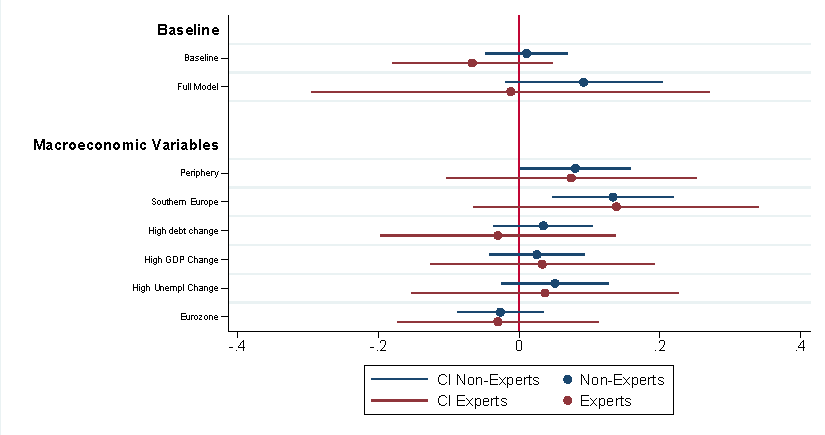
\includegraphics[scale=0.65]{QuestionS_1504.pdf}
    \footnotesize{
     \subcaption{Question 5.4}}
    \label{fig:my_label}
    \end{minipage}
     \begin{minipage}{0.5\textwidth}
    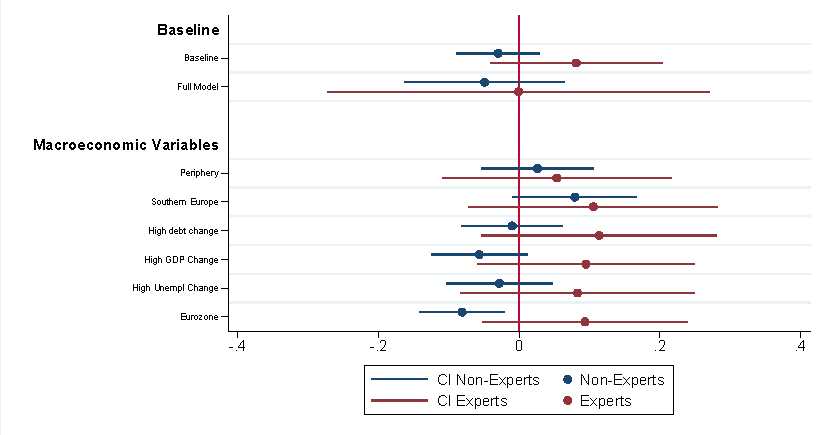
\includegraphics[scale=0.65]{QuestionS_1505.pdf}
    \footnotesize{
     \subcaption{Question 5.5}}
    \label{fig:my_label}
    \end{minipage}
     \begin{minipage}{0.5\textwidth}
    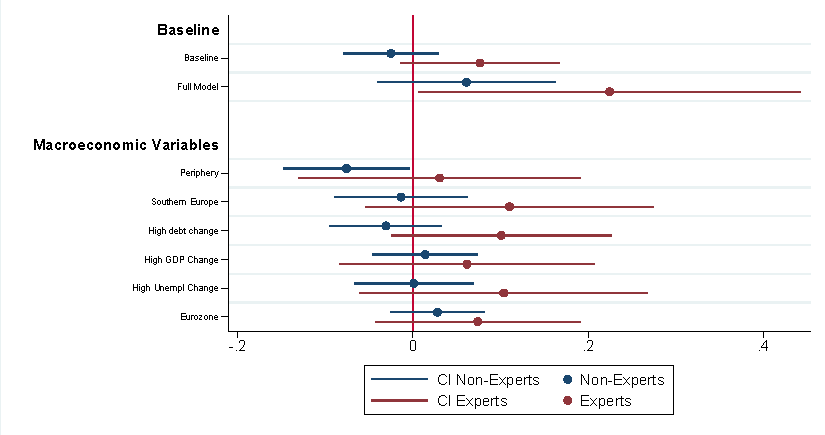
\includegraphics[scale=0.65]{QuestionS_1506.pdf}
    \footnotesize{
     \subcaption{Question 5.6}}
    \label{fig:my_label}
    \end{minipage}
    \vskip 0.3cm
        \tiny
     \tablenotes{Question 5.1: The rescue experience made many citizens in the borrower countries feel guilty; Question 5.2: The rescue experience made many citizens in the borrower countries feel exploited; Question 5.3: The rescue experience made many citizens in the borrower countries feel inferior; Question 5.4: The rescue experience made many citizens in the lender countries feel exploited; Question 5.5 The rescue experience made many citizens in the lender countries feel disappointed; Question 5.6: The rescue experience strengthened friendships between citizens; Question 7: Greece will fully pay back it's debt}
\end{figure} 

\begin{figure}[h!]
\caption{Driving force and beneficiaries of the program}
    \begin{minipage}{0.5\textwidth}
    
    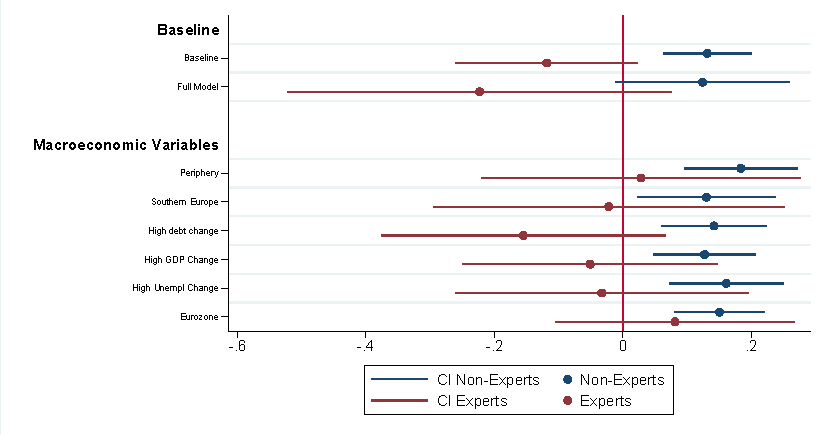
\includegraphics[scale=0.65]{QuestionS_1301.pdf}
    \footnotesize{
     \subcaption{Question 3} }
\end{minipage}
\begin{minipage}{0.5\textwidth}
    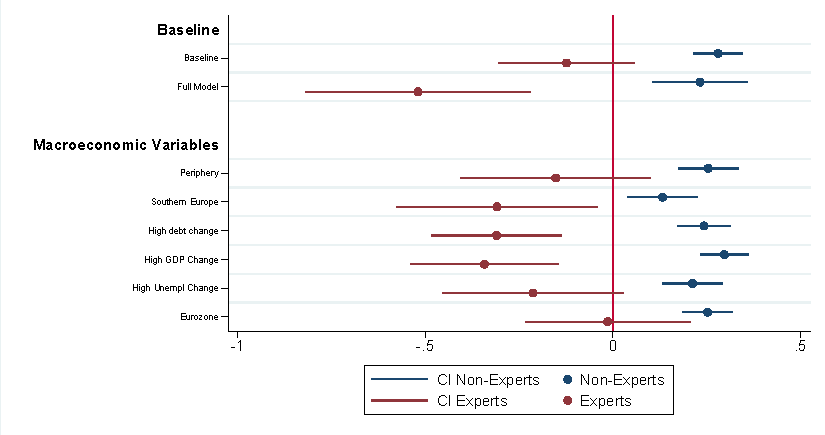
\includegraphics[scale=0.65]{QuestionS_1401.pdf}
    \footnotesize{
      \subcaption{Question 4}
      }
\end{minipage} 
 \begin{minipage}{0.5\textwidth}
  
    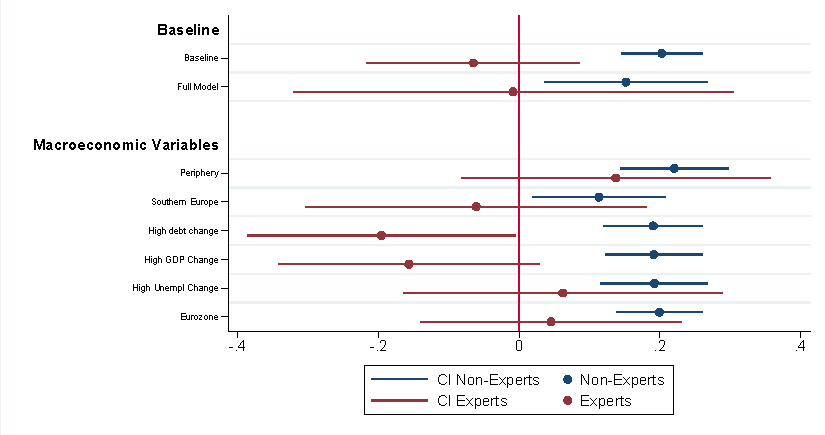
\includegraphics[scale=0.65]{QuestionS_1701.pdf}
    \footnotesize{
     \subcaption{Question 7}}
    \label{fig:my_label}
    \end{minipage}
    \vskip 0.3cm
        \tiny
    \tablenotes{Question 3: Who was the driving force behind signing the memorandum; Question 4: Who was the main beneficiary of the program; Question 7: Who primarily benefited from the loans to Greece}
\end{figure} 










